\chapter{Stock Option Plan Model}

\section{Introduction}

Stock option plans are a pool of shares that are reserved to be granted as stock options to employees. Simply put, a stock option gives the right (but not the obligation) to buy a certain amount of stock at a certain price. As the stock appreciates, the stock options become more valuable.

To make it more concrete to the reader, a typical stock option contract might look like the following:

\begin{figure}[h!]
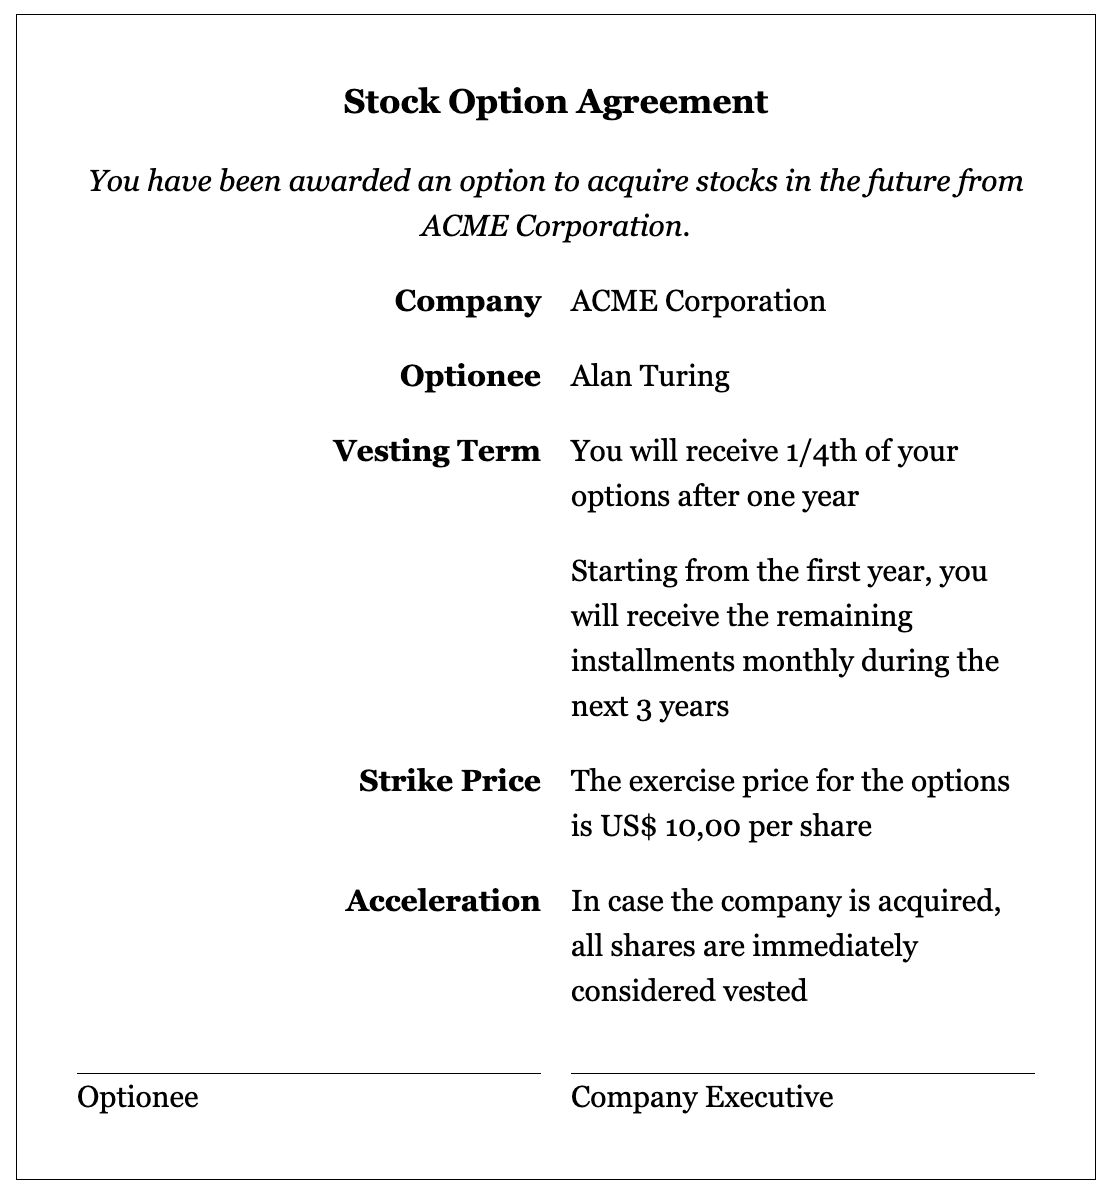
\includegraphics[width=\textwidth]{pics/sopa.png}
\caption{Example of a stock option contract}
\label{fig:stock_option_contract}
\end{figure}

The Stock Option Plan Model is a formal representation of stock option plans used by companies to incentivize employees and other stakeholders. 
\section{Model Design}

The model is designed around signatures that represent the stock option plan, the security that represents stock options issued from that stock option plan, the transactions that issue stock options, and the transactions that exercise stock options. In the OCF, an event is registered whenever new shares are vested (become available for exercises). 

In our model, we leverage Alloy's higher-arity relations to directly give the number of shares that are vested at a given date.

\section{Signatures}

\subsection{Stock Plan Signature}

First and foremost, all stock option plans have a number of reserved shares. Indeed, a stock option plan is sometimes called an option pool\cite{investopediaOptionPool}.

From the stock option plan, stock option grants will be awarded as securities, and, as those options became available to optionees (vested), they can be exercised\cite{investopediaExerciseDefinition}. We include relations to exercises and securities in the stock option plan signature to aid in navigating the model.

\begin{listing}[!h]
\begin{minted}{alloy}
sig StockPlan {
    reservedShares : one Int,
    exercises : disj set Exercise,
    securities : disj set Security
}
\end{minted}
\caption{The \texttt{StockPlan} signature}
\label{lst:stock-plan-signature-2}
\end{listing}


The \verb|disj| modifiers are used so that every exercise and security are unique to a stock option plan.

\subsection{The Security Signature}

The security signature represents a security that is issued from a stock option plan. The security has a number of shares, and a reference to the stock option plan from which it was issued, as well as to the vesting term object that define its vesting schedule.

\begin{listing}[!h]
\begin{minted}{alloy}
sig Security {
    vestingTerm : disj one VestingTerm,
    shares : one Int,
    stockPlan : one StockPlan,
}
\end{minted}
\caption{The \texttt{Security} signature}
\label{lst:security-signature-2}
\end{listing}


Since each \verb|VestingTerm| is exclusive to a \verb|Security|, we use the \verb|disj| modifier. Since a \verb|StockPlan| has many securities, it is not necessary to make the relation disjoint.

\subsection{Issuance signature}

The issuance signature is the transaction that creates a new stock option from a stock option plan. It refers to the newly issued \verb|Security|. It also assigns a \verb|VestingTerm| to the \verb|Security|, which defines the vesting schedule for the security.

\noindent\todo{Perhaps the disj modifier here is superfluous}

\begin{listing}[!h]
\begin{minted}{alloy}
		sig Issuance {
			security : disj one Security,
			shares : one Int,
			vestingTerm : disj one VestingTerm,
			stockPlan : one StockPlan
		}
\end{minted}
\caption{The \texttt{Issuance} signature}
\label{lst:issuance-signature-2}
\end{listing}


\subsection{Exercise signature}

As shares become vested according to the vesting term, the optionee is able to exercise those options into actual shares. A resulting security is thus created. Exercises can be many, as long as the total number of exercised shares does not exceed the total number of vested shares.

\begin{listing}[!h]
\begin{minted}{alloy}
		sig Exercise {
			security : one Security,
			resultingSecurity : one Security,
			stockPlan : one StockPlan,
			shares : one Int
			} { pos[shares] }
\end{minted}
\caption{The \texttt{Exercise} signature}
\label{lst:exercise-signature-2}
\end{listing}


The \verb|pos[shares]| constraint ensures that the number of exercised shares is always positive. This excludes the uneffectful exercise of zero shares.

\subsection{Vesting Term signature}

As regards the stock option plan model, we adopt a simplified version of the vesting term, without loss of generality. In this case, we model the vesting term as having higher-arity relation mapping numbers of shares to status of vesting. 

\begin{listing}[!h]
\begin{minted}{alloy}
sig VestingTerm {
    security : one Security,
    vestingConditions : set Status -> one Int
}

enum Status { Vested, Pending }
\end{minted}
\caption{The \texttt{VestingTerm} signature}
\label{lst:vesting-term-signature-2}
\end{listing}


\section{Functions (Queries)}

Since our focus here is on respecting accounting principles, we define functions that allow us to calculate the numbers of vested shares, and from that point we can constrain the model to respect the accounting principles.

\begin{listing}[!h]
\begin{minted}{alloy}
fun vestedShares[v : VestingTerm] : one Int {
    sum[v.vestingConditions[Vested]]
}

fun pendingShares[v : VestingTerm] : one Int {
    sum[v.vestingConditions[Pending]]
}

fun exercisedShares[v : VestingTerm] : one Int {
    let es = { e : Exercise | e.security = v.security } |
    sum[es.shares]
}
\end{minted}
\caption{The \texttt{vestedShares}, \texttt{pendingShares}, and \texttt{exercisedShares} functions}
\label{lst:vested-shares-function-2}
\end{listing}


Even though Alloy is not aimed at arithmetic modeling, because ints are restricted to relatively small bit-width, we can use them to model the vesting term as a function that maps the number of vested shares to the status of vesting.

\section{Constraints}

\subsection{All shares must be positive in the signatures}

\begin{listing}[!h]
\begin{minted}{alloy}
fact {
    all s : Security | pos[s.shares]
    all i : Issuance | pos[i.shares]
    all e : Exercise | pos[e.shares]
}
\end{minted}
\caption{The \texttt{shares} constraint}
\label{lst:shares-constraint-2}
\end{listing}


\subsection{Relational constraints}

These constraints are useful to ensure that the bi-directional relations are really inverses. This is a very idiomatic way of constraining the model, and it is very useful to ensure that the model is well-formed.

\begin{listing}[!h]
\begin{minted}{alloy}
fact { 
    stockPlan = ~securities 
}

fact {
    ~security = vestingTerm
}
\end{minted}
\caption{The \texttt{relational} constraints}
\label{lst:relational-constraints-2}
\end{listing}


\subsection{Accounting equations}

This is at the heart of the stock option plan system, and it is something that JSON Schema can not hope to express. We can constrain the model so that it is not possible to over-vest or over-exercise shares.

\begin{listing}[!h]
\begin{minted}{alloy}  
fact {
    all s : Security |
    gte[s.shares, sum[s.vestingTerm.vestingConditions[Status]]]
}
\end{minted}
\caption{The \texttt{vesting} constraint}
\label{lst:vesting-constraint-2}
\end{listing}


This makes sure that share numbers are not over-vested.

\begin{listing}[!h]
\begin{minted}{alloy}
fact { 
    all v : VestingTerm | lte[v.exercisedShares, v.vestedShares] 
}
\end{minted}
\caption{The \texttt{exercise} constraint}
\label{lst:exercise-constraint-2}
\end{listing}


This makes sure that share numbers are not over-exercised.

